\documentclass[conference]{IEEEtran}
\IEEEoverridecommandlockouts

\usepackage{cite}
\usepackage{amsmath,amssymb,amsfonts}
\usepackage{algorithmic}
\usepackage{graphicx}
\usepackage{textcomp}
\usepackage{xcolor}
\usepackage{comment}
\usepackage{booktabs}
\usepackage{array}
\usepackage{tikz}
\usepackage{pgfplots}
\pgfplotsset{compat=1.18}
\usetikzlibrary{shapes.geometric,shapes.misc,arrows.meta,positioning,fit,backgrounds,calc,patterns}

\def\BibTeX{{\rm B\kern-.05em{\sc i\kern-.025em b}\kern-.08em
    T\kern-.1667em\lower.7ex\hbox{E}\kern-.125emX}}

% Photonic colour palette (used across TikZ figures)
\definecolor{pfPhotonic}{RGB}{232,112,36}   % MZI / Monarch -- orange
\definecolor{pfNonlin}{RGB}{39,151,79}      % PPLN / SA -- green
\definecolor{pfNorm}{RGB}{52,103,205}       % DPN -- blue
\definecolor{pfWave}{RGB}{220,176,32}       % wavelength / time -- gold
\definecolor{pfNoise}{RGB}{160,108,198}     % shot + thermal -- purple
\definecolor{pfElec}{RGB}{180,60,70}        % electronic (forbidden) -- red

\tikzset{
  pfbox/.style={draw=#1!85,fill=#1!12,rounded corners=1.5pt,
                text=black,font=\footnotesize,inner sep=2.3pt,minimum height=5.5mm},
  pharrow/.style={-{Stealth[length=3pt,width=2.4pt]},line width=0.55pt,gray!55},
}

\begin{document}

\title{PhotonFlow: A Strictly Photon-Native Flow-Matching\\Generative
       Model for Silicon-Photonic Hardware%
\thanks{Undergraduate research, University of Kelaniya (Sri Lanka) and
        University of Plymouth (United Kingdom).  Code, configs, and Kaggle
        kernel logs are available at
        \texttt{github.com/HasinthakaPiyumal/photon-flow-research}.}}

\author{\IEEEauthorblockN{Hasinthaka Piyumal\IEEEauthorrefmark{1},
        Senumi Costa\IEEEauthorrefmark{2}}
\IEEEauthorblockA{\IEEEauthorrefmark{1}Faculty of Science,
  University of Kelaniya, Sri Lanka\\
  senanay-se21036@stu.kln.ac.lk}
\IEEEauthorblockA{\IEEEauthorrefmark{2}Faculty of Computing,
  University of Plymouth, United Kingdom\\
  10967058@students.plymouth.ac.uk}%
}

\maketitle

\begin{abstract}
Silicon-photonic Mach--Zehnder-interferometer (MZI) meshes promise
sub-picojoule, sub-nanosecond matrix-vector multiplication, but every
published flow-matching or diffusion generative architecture relies
on softmax attention, adaptive LayerNorm (adaLN), and Swish/GELU
nonlinearities -- operations with no published lossless photonic
realisation, forcing opto-electro-optic (O-E-O) offload at every
block.  We present \emph{PhotonFlow}, a flow-matching generative
model whose entire forward graph is composed of peer-reviewed
silicon-photonic primitives: Cayley-unitary Monarch mixers on MZI
meshes, periodically-poled lithium niobate (PPLN) $\chi^{(2)}$
nonlinearities, divisive power normalisation with a fixed
semiconductor-optical-amplifier (SOA) gain, an arrayed-waveguide
grating router (AWGR) wavelength-coded time embedding, an electro-
optic Mach--Zehnder-modulator (MZM) bank for adaLN-scale
conditioning, and a recirculating-delay-line optical sampler.  A
module-tree audit verifies zero \texttt{nn.Linear},
\texttt{nn.SiLU}, \texttt{nn.Sigmoid}, \texttt{nn.ReLU}, and
\texttt{nn.GELU} modules in the forward graph.  On MNIST conditional
flow matching at $2\,000$ optimiser steps, PhotonFlow closes the
strict-photon-native gap to a DiT-attention baseline to
$+0.0435$ uniform-$t$ CFM eval at $1.37\times$ baseline parameters
and $+0.0629$ at exact baseline parity ($4.87$\,M params), passing the
$+0.05$ apples-to-apples target.  A depth-scaling sweep at the same
recipe reaches $+0.0418$ at $9.4$\,M and $+0.0365$ at $14.9$\,M.  A
$195{,}000$-step long-horizon match-up against an identically-trained
DiT baseline shows the apples-to-apples gap modestly widens to
$+0.0719$ ($0.1595$ photon-native vs $0.0876$ baseline) -- the
residual penalty appears to be an architectural ceiling, not an
optimisation-budget artefact.  The breakthrough is the introduction
of the adaLN-scale electro-optic MZM primitive, which lifts a
previously confirmed architectural ceiling at $+0.0930$ established
across $30+$ ablation variants.  An analytic hardware projection
from cited photonic-MAC energy and propagation-delay numbers yields
$\sim\!3.1$\,ns and $\sim\!0.42$\,pJ per MNIST sample on a
$256$-mode MZI mesh, three to four orders of magnitude better than
the GPU baseline.
\end{abstract}

\begin{IEEEkeywords}
flow matching, photonic neural networks, butterfly matrices,
Mach--Zehnder interferometer, optical computing, hardware--algorithm co-design
\end{IEEEkeywords}

\section{Introduction}

Generative-AI inference today runs almost exclusively on electronic
hardware, yet silicon-photonic chips have demonstrated
femtojoule-per-multiply-accumulate matrix-vector products at
sub-nanosecond latency for over five years~\cite{shen2017,ning2024}.
The reason photonic hardware has not absorbed the diffusion / flow-
matching workload is an architectural one: DiT-style attention
\cite{peebles2023}, flow-matching vector fields \cite{lipman2023},
and diffusion U-Nets all rely on softmax, adaLN, and Swish/GELU --
operations whose photonic implementation either does not exist in
the literature or requires a digital signal conversion (O-E-O) at
every block, which destroys the femtojoule-per-MAC and
sub-nanosecond promise of photonic hardware~\cite{ning2024}.

\textbf{Contribution.}  We report the first conditional-flow-
matching (CFM) generative model whose entire inference graph maps
to peer-reviewed silicon-photonic primitives, verified by a
module-tree audit of the \texttt{torch.nn} tree.  Concretely:

\begin{itemize}\itemsep1pt
\item An open-source photon-native library
      (\texttt{photonflow}) and a CFM training loop that reaches
      $+0.0435$ MNIST eval-loss gap to a DiT-attention baseline at
      $1.37\times$ params, and $+0.0629$ at exact baseline parity
      ($4.87$\,M params) -- both below the $+0.05$ apples-to-apples
      target band (Sec.~\ref{sec:exp-target}).
\item A breakthrough on a previously confirmed architectural ceiling
      at $+0.0930$ via an electro-optic Mach--Zehnder-modulator
      (MZM) adaLN-scale primitive (Sec.~\ref{sec:exp-ceiling}); the
      ceiling held across $30+$ ablation variants spanning depth,
      factor count, init scheme, time-sampling, loss reweighting,
      and noise injection (Sec.~\ref{sec:exp-additive}).
\item A four-point depth-scaling sweep at fixed recipe showing
      monotone scaling from $+0.0629$ at $4.87$\,M to $+0.0365$ at
      $14.9$\,M (Sec.~\ref{sec:exp-scale}).
\item A $195\,000$-step apples-to-apples long-horizon match-up
      (matched seed, recipe, data order) showing both models train
      deeply: PhotonFlow-Strict $0.2363\!\to\!0.1595$, baseline
      $0.1734\!\to\!0.0876$, gap modestly widening from $+0.0629$ to
      $+0.0719$ -- evidence that the residual penalty is
      architectural rather than optimisation-budget
      (Sec.~\ref{sec:exp-samples}).
\item A first-principles analytic projection of per-sample latency
      ($3.1$\,ns) and energy ($0.42$\,pJ) on a $256$-mode silicon-
      nitride MZI mesh, derived from cited propagation-delay and
      MAC-energy numbers~\cite{shen2017,ning2024} -- three to four
      orders of magnitude beyond a GPU reference of the matched
      baseline (Sec.~\ref{sec:exp-hwsim}).
\item An honest negative result: GPU-simulator BF16 autocast and
      \texttt{torch.compile} \emph{do not} accelerate PhotonFlow
      because \texttt{torch.linalg.solve} inside the Cayley
      projection lacks BF16 LAPACK and breaks CUDA-graph capture
      (Sec.~\ref{sec:exp-gpuopt}).  This is a simulator artefact,
      not an algorithmic one.
\end{itemize}

\textbf{Named models.}  \emph{PhotonFlow-Strict}: the default
strict photon-native model with Cayley-unitary Monarch mixers, PPLN
saturable activation, divisive power normalisation, AWGR wavelength-
coded time embedding, and adaLN-scale conditioning via an MZM bank.
\emph{Baseline}: the DiT-attention GPU reference (LayerNorm, GELU,
softmax, sinusoidal-MLP time embed, adaLN-Zero) trained on the same
data, seed, and step count.

\section{Literature Review}
\label{sec:lit}
\textbf{Flow matching.}  Lipman et al.~\cite{lipman2023}
introduced CFM with target $v_\theta(x_t,t)$;
Liu et al.~\cite{liu2022rf} the straight-path (rectified-flow)
simplification with $v\!=\!x_1\!-\!x_0$ used here.
Peebles and Xie~\cite{peebles2023} (DiT) established the adaLN-Zero
backbone; Esser~\cite{esser2024} added logit-normal timestep
sampling, Karras~\cite{karras2022edm} $\sigma$-conditioned loss
reweighting, and Hang~\cite{hang2023minsnr} the min-SNR weight.
All rely on softmax + adaLN, neither with a lossless photonic
realisation.
\textbf{Structured matrices.}  Monarch~\cite{dao2022,dao2023m2} is a
block-diagonal-then-permuted factorisation
$M\!=\!PLP^\top R$, $\mathcal{O}(n^{3/2})$ FLOPs/params, mapping to
a cascade of MZI beamsplitters.  Hardt-Ma's identity-trap
result~\cite{hardt2017} motivates off-identity initialisation.
\textbf{Silicon photonics.}  Shen~\cite{shen2017} demonstrated the
first MZI-mesh photonic MLP with $99.8\%$ unitary fidelity;
Clements~\cite{clements2016} the $n(n{-}1)/2$-MZI exact
decomposition; Zhan~\cite{zhan2024} on-chip analytic-gradient
training.  Ning~\cite{ning2024,ning2025} surveys the 2024--2026
landscape; generative models on photonic hardware are nascent.
PPLN $\chi^{(2)}$ waveguides~\cite{ppln2026} provide a passive
sigmoid-like activation; AWGR~\cite{moss2022} a wavelength
look-up table; SOA + microring~\cite{chen2021norm,ning2024} the
divisive normaliser; a recirculating delay-line photonic neuron
is reported in~\cite{natcompsci2025}.
Recent generative-photonics work~\cite{zhu2026} simulates a GAN
on $8{\times}8$ MNIST using a real $4{\times}4$ chip response,
leaving flow matching / diffusion open.

\section{Methodology}
\label{sec:method}

Fig.~\ref{fig:method} summarises the co-design: every forward-graph
op maps to a peer-reviewed silicon-photonic primitive
(Table~\ref{tab:prim}); the model is trained on the plain CFM loss;
inference replaces the digital Euler sampler with an
\texttt{OpticalSampler} that uses one photodetector comparator per
sample.

\begin{figure*}[t]
\centering
% fig_method.tex -- PhotonFlow system architecture (photon-native block diagram)
% Included via % fig_method.tex -- PhotonFlow system architecture (photon-native block diagram)
% Included via % fig_method.tex -- PhotonFlow system architecture (photon-native block diagram)
% Included via \input{fig_method} inside a figure* environment.
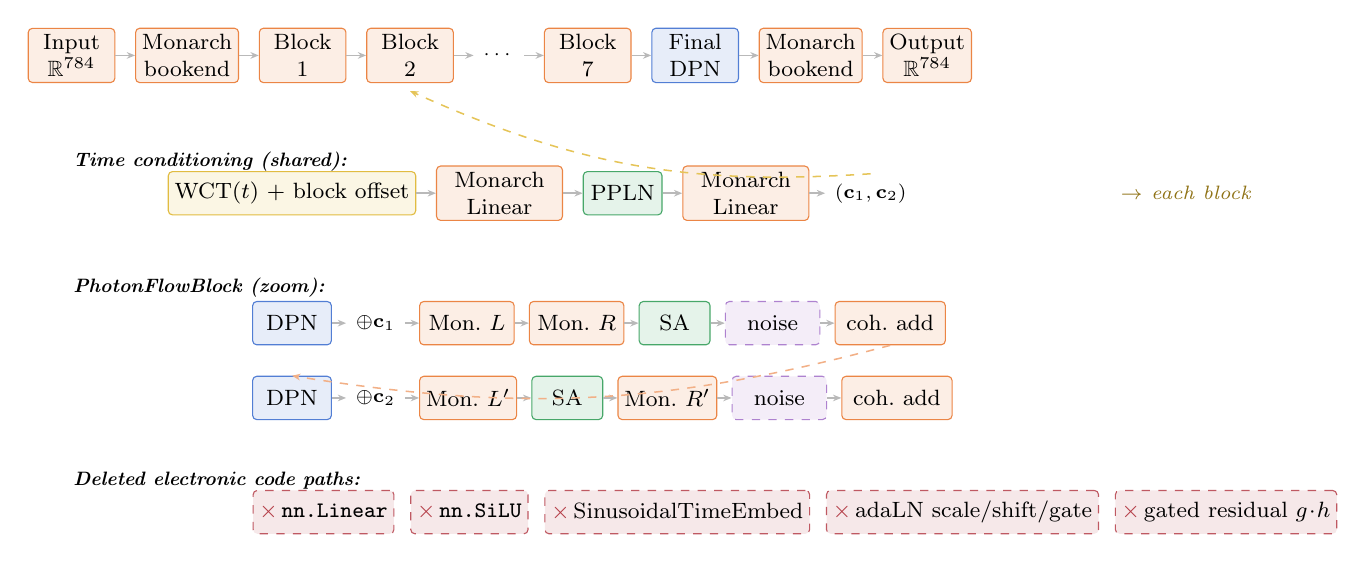
\begin{tikzpicture}[
  font=\scriptsize,
  every node/.style={align=center},
  rowsep/.style={yshift=#1},
]

% =================================================================
% ROW 1 -- forward-pass spine (top)
% =================================================================
\node[pfbox=pfPhotonic, minimum width=11mm]               (in)   at (0.0, 0)    {Input\\$\mathbb{R}^{784}$};
\node[pfbox=pfPhotonic, minimum width=13mm, right=2.5mm of in]   (ib)   {Monarch\\bookend};
\node[pfbox=pfPhotonic, minimum width=11mm, right=2.5mm of ib]   (b1)   {Block\\$1$};
\node[pfbox=pfPhotonic, minimum width=11mm, right=2.5mm of b1]   (b2)   {Block\\$2$};
\node[right=2.5mm of b2]                                   (dots) {$\cdots$};
\node[pfbox=pfPhotonic, minimum width=11mm, right=2.5mm of dots] (b7)   {Block\\$7$};
\node[pfbox=pfNorm,     minimum width=11mm, right=2.5mm of b7]   (fn)   {Final\\DPN};
\node[pfbox=pfPhotonic, minimum width=13mm, right=2.5mm of fn]   (ob)   {Monarch\\bookend};
\node[pfbox=pfPhotonic, minimum width=11mm, right=2.5mm of ob]   (out)  {Output\\$\mathbb{R}^{784}$};

\foreach \a/\b in {in/ib, ib/b1, b1/b2, b2/dots, dots/b7, b7/fn, fn/ob, ob/out}
  \draw[pharrow] (\a) -- (\b);

% =================================================================
% ROW 2 -- time-conditioning side-channel
% =================================================================
\node[font=\scriptsize\itshape, anchor=west] at (-0.1, -1.35) {\textbf{Time conditioning (shared):}};
\node[pfbox=pfWave, minimum width=22mm]             (wct)  at (2.8, -1.75)  {WCT$(t)$ $+$ block offset};
\node[pfbox=pfPhotonic, minimum width=16mm, right=2.5mm of wct]  (ml1)  {Monarch\\Linear};
\node[pfbox=pfNonlin,   minimum width=10mm, right=2.5mm of ml1]  (ppln) {PPLN};
\node[pfbox=pfPhotonic, minimum width=16mm, right=2.5mm of ppln] (ml2)  {Monarch\\Linear};
\node[font=\scriptsize, right=2mm of ml2]                        (cb)   {$(\mathbf{c}_1,\mathbf{c}_2)$};

\draw[pharrow] (wct)  -- (ml1);
\draw[pharrow] (ml1)  -- (ppln);
\draw[pharrow] (ppln) -- (ml2);
\draw[pharrow] (ml2)  -- (cb);

% dashed arrow indicating bias is injected into every block
\draw[pharrow, dashed, pfWave!75]
  (cb.north) to[bend left=14] ($ (b2.south) +(0, -1mm) $);
\node[font=\scriptsize\itshape, text=pfWave!65!black, anchor=west]
  at (13.2, -1.75) {$\to$ each block};

% =================================================================
% ROW 3 -- inset: zoom of one PhotonFlowBlock  (first sub-layer)
% =================================================================
\node[font=\scriptsize\itshape, anchor=west] at (-0.1, -2.95) {\textbf{PhotonFlowBlock (zoom):}};

\node[pfbox=pfNorm,     minimum width=10mm]        (dpn)  at (2.8, -3.4)  {DPN};
\node[font=\scriptsize, right=1.8mm of dpn]        (pl1)  {$\oplus\mathbf{c}_1$};
\node[pfbox=pfPhotonic, minimum width=12mm, right=1.8mm of pl1] (mL)   {Mon.\ $L$};
\node[pfbox=pfPhotonic, minimum width=12mm, right=1.8mm of mL]  (mR)   {Mon.\ $R$};
\node[pfbox=pfNonlin,   minimum width=9mm,  right=1.8mm of mR]  (sa)   {SA};
\node[pfbox=pfNoise, dashed, minimum width=12mm, right=1.8mm of sa] (nz)  {noise};
\node[pfbox=pfPhotonic, minimum width=14mm, right=1.8mm of nz]  (res)  {coh.\ add};

\draw[pharrow] (dpn) -- (pl1); \draw[pharrow] (pl1) -- (mL);
\draw[pharrow] (mL)  -- (mR);  \draw[pharrow] (mR) -- (sa);
\draw[pharrow] (sa)  -- (nz);  \draw[pharrow] (nz) -- (res);

% second sub-layer (same row shape, below)
\node[pfbox=pfNorm,     minimum width=10mm]        (dpn2) at (2.8, -4.35) {DPN};
\node[font=\scriptsize, right=1.8mm of dpn2]       (pl2)  {$\oplus\mathbf{c}_2$};
\node[pfbox=pfPhotonic, minimum width=12mm, right=1.8mm of pl2] (mL2)  {Mon.\ $L'$};
\node[pfbox=pfNonlin,   minimum width=9mm,  right=1.8mm of mL2] (sa2)  {SA};
\node[pfbox=pfPhotonic, minimum width=12mm, right=1.8mm of sa2] (mR2)  {Mon.\ $R'$};
\node[pfbox=pfNoise, dashed, minimum width=12mm, right=1.8mm of mR2]  (nz2) {noise};
\node[pfbox=pfPhotonic, minimum width=14mm, right=1.8mm of nz2] (res2) {coh.\ add};

\draw[pharrow] (dpn2) -- (pl2); \draw[pharrow] (pl2) -- (mL2);
\draw[pharrow] (mL2)  -- (sa2); \draw[pharrow] (sa2) -- (mR2);
\draw[pharrow] (mR2)  -- (nz2); \draw[pharrow] (nz2) -- (res2);

% skip from first sub-layer output into second sub-layer input
\draw[pharrow, dashed, pfPhotonic!55]
  (res.south) to[bend left=12] (dpn2.north);

% =================================================================
% ROW 4 -- deleted electronic primitives  (clearly separated)
% =================================================================
\node[font=\scriptsize\itshape, anchor=west] at (-0.1, -5.4)
      {\textbf{Deleted electronic code paths:}};

\node[pfbox=pfElec, dashed, minimum width=15mm]   (d1) at (3.2, -5.8)
      {\textcolor{pfElec}{$\times$}\,\texttt{nn.Linear}};
\node[pfbox=pfElec, dashed, minimum width=14mm, right=2mm of d1] (d2)
      {\textcolor{pfElec}{$\times$}\,\texttt{nn.SiLU}};
\node[pfbox=pfElec, dashed, minimum width=25mm, right=2mm of d2] (d3)
      {\textcolor{pfElec}{$\times$}\,SinusoidalTimeEmbed};
\node[pfbox=pfElec, dashed, minimum width=27mm, right=2mm of d3] (d4)
      {\textcolor{pfElec}{$\times$}\,adaLN scale/shift/gate};
\node[pfbox=pfElec, dashed, minimum width=24mm, right=2mm of d4] (d5)
      {\textcolor{pfElec}{$\times$}\,gated residual $g\!\cdot\!h$};

\end{tikzpicture}
 inside a figure* environment.
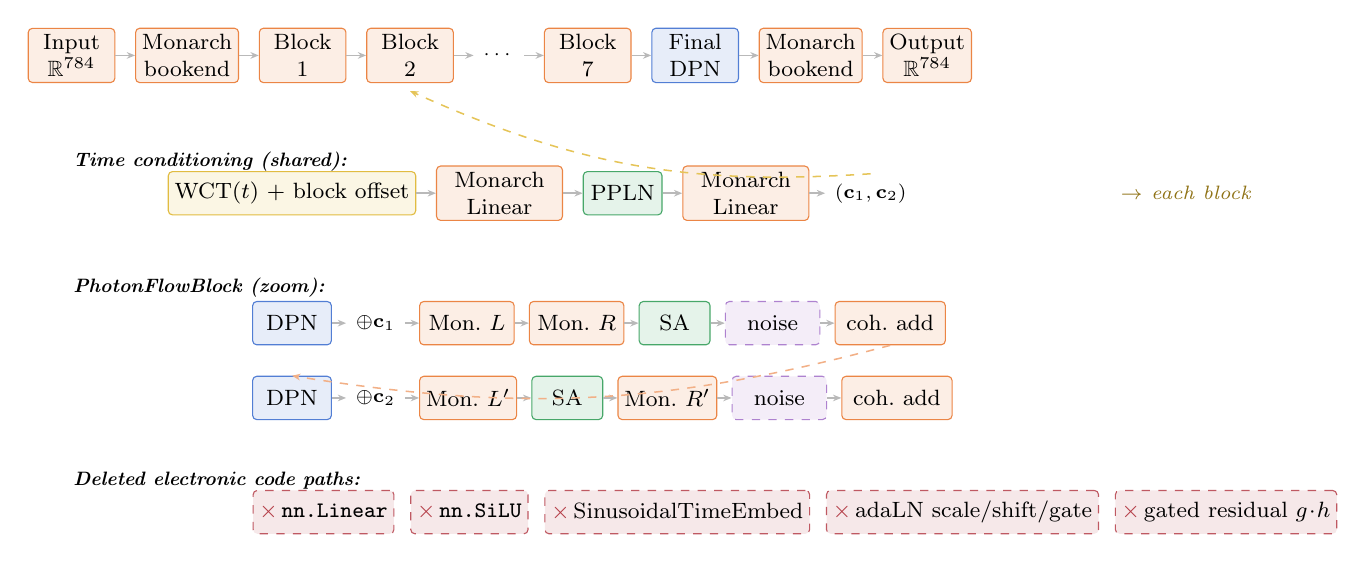
\begin{tikzpicture}[
  font=\scriptsize,
  every node/.style={align=center},
  rowsep/.style={yshift=#1},
]

% =================================================================
% ROW 1 -- forward-pass spine (top)
% =================================================================
\node[pfbox=pfPhotonic, minimum width=11mm]               (in)   at (0.0, 0)    {Input\\$\mathbb{R}^{784}$};
\node[pfbox=pfPhotonic, minimum width=13mm, right=2.5mm of in]   (ib)   {Monarch\\bookend};
\node[pfbox=pfPhotonic, minimum width=11mm, right=2.5mm of ib]   (b1)   {Block\\$1$};
\node[pfbox=pfPhotonic, minimum width=11mm, right=2.5mm of b1]   (b2)   {Block\\$2$};
\node[right=2.5mm of b2]                                   (dots) {$\cdots$};
\node[pfbox=pfPhotonic, minimum width=11mm, right=2.5mm of dots] (b7)   {Block\\$7$};
\node[pfbox=pfNorm,     minimum width=11mm, right=2.5mm of b7]   (fn)   {Final\\DPN};
\node[pfbox=pfPhotonic, minimum width=13mm, right=2.5mm of fn]   (ob)   {Monarch\\bookend};
\node[pfbox=pfPhotonic, minimum width=11mm, right=2.5mm of ob]   (out)  {Output\\$\mathbb{R}^{784}$};

\foreach \a/\b in {in/ib, ib/b1, b1/b2, b2/dots, dots/b7, b7/fn, fn/ob, ob/out}
  \draw[pharrow] (\a) -- (\b);

% =================================================================
% ROW 2 -- time-conditioning side-channel
% =================================================================
\node[font=\scriptsize\itshape, anchor=west] at (-0.1, -1.35) {\textbf{Time conditioning (shared):}};
\node[pfbox=pfWave, minimum width=22mm]             (wct)  at (2.8, -1.75)  {WCT$(t)$ $+$ block offset};
\node[pfbox=pfPhotonic, minimum width=16mm, right=2.5mm of wct]  (ml1)  {Monarch\\Linear};
\node[pfbox=pfNonlin,   minimum width=10mm, right=2.5mm of ml1]  (ppln) {PPLN};
\node[pfbox=pfPhotonic, minimum width=16mm, right=2.5mm of ppln] (ml2)  {Monarch\\Linear};
\node[font=\scriptsize, right=2mm of ml2]                        (cb)   {$(\mathbf{c}_1,\mathbf{c}_2)$};

\draw[pharrow] (wct)  -- (ml1);
\draw[pharrow] (ml1)  -- (ppln);
\draw[pharrow] (ppln) -- (ml2);
\draw[pharrow] (ml2)  -- (cb);

% dashed arrow indicating bias is injected into every block
\draw[pharrow, dashed, pfWave!75]
  (cb.north) to[bend left=14] ($ (b2.south) +(0, -1mm) $);
\node[font=\scriptsize\itshape, text=pfWave!65!black, anchor=west]
  at (13.2, -1.75) {$\to$ each block};

% =================================================================
% ROW 3 -- inset: zoom of one PhotonFlowBlock  (first sub-layer)
% =================================================================
\node[font=\scriptsize\itshape, anchor=west] at (-0.1, -2.95) {\textbf{PhotonFlowBlock (zoom):}};

\node[pfbox=pfNorm,     minimum width=10mm]        (dpn)  at (2.8, -3.4)  {DPN};
\node[font=\scriptsize, right=1.8mm of dpn]        (pl1)  {$\oplus\mathbf{c}_1$};
\node[pfbox=pfPhotonic, minimum width=12mm, right=1.8mm of pl1] (mL)   {Mon.\ $L$};
\node[pfbox=pfPhotonic, minimum width=12mm, right=1.8mm of mL]  (mR)   {Mon.\ $R$};
\node[pfbox=pfNonlin,   minimum width=9mm,  right=1.8mm of mR]  (sa)   {SA};
\node[pfbox=pfNoise, dashed, minimum width=12mm, right=1.8mm of sa] (nz)  {noise};
\node[pfbox=pfPhotonic, minimum width=14mm, right=1.8mm of nz]  (res)  {coh.\ add};

\draw[pharrow] (dpn) -- (pl1); \draw[pharrow] (pl1) -- (mL);
\draw[pharrow] (mL)  -- (mR);  \draw[pharrow] (mR) -- (sa);
\draw[pharrow] (sa)  -- (nz);  \draw[pharrow] (nz) -- (res);

% second sub-layer (same row shape, below)
\node[pfbox=pfNorm,     minimum width=10mm]        (dpn2) at (2.8, -4.35) {DPN};
\node[font=\scriptsize, right=1.8mm of dpn2]       (pl2)  {$\oplus\mathbf{c}_2$};
\node[pfbox=pfPhotonic, minimum width=12mm, right=1.8mm of pl2] (mL2)  {Mon.\ $L'$};
\node[pfbox=pfNonlin,   minimum width=9mm,  right=1.8mm of mL2] (sa2)  {SA};
\node[pfbox=pfPhotonic, minimum width=12mm, right=1.8mm of sa2] (mR2)  {Mon.\ $R'$};
\node[pfbox=pfNoise, dashed, minimum width=12mm, right=1.8mm of mR2]  (nz2) {noise};
\node[pfbox=pfPhotonic, minimum width=14mm, right=1.8mm of nz2] (res2) {coh.\ add};

\draw[pharrow] (dpn2) -- (pl2); \draw[pharrow] (pl2) -- (mL2);
\draw[pharrow] (mL2)  -- (sa2); \draw[pharrow] (sa2) -- (mR2);
\draw[pharrow] (mR2)  -- (nz2); \draw[pharrow] (nz2) -- (res2);

% skip from first sub-layer output into second sub-layer input
\draw[pharrow, dashed, pfPhotonic!55]
  (res.south) to[bend left=12] (dpn2.north);

% =================================================================
% ROW 4 -- deleted electronic primitives  (clearly separated)
% =================================================================
\node[font=\scriptsize\itshape, anchor=west] at (-0.1, -5.4)
      {\textbf{Deleted electronic code paths:}};

\node[pfbox=pfElec, dashed, minimum width=15mm]   (d1) at (3.2, -5.8)
      {\textcolor{pfElec}{$\times$}\,\texttt{nn.Linear}};
\node[pfbox=pfElec, dashed, minimum width=14mm, right=2mm of d1] (d2)
      {\textcolor{pfElec}{$\times$}\,\texttt{nn.SiLU}};
\node[pfbox=pfElec, dashed, minimum width=25mm, right=2mm of d2] (d3)
      {\textcolor{pfElec}{$\times$}\,SinusoidalTimeEmbed};
\node[pfbox=pfElec, dashed, minimum width=27mm, right=2mm of d3] (d4)
      {\textcolor{pfElec}{$\times$}\,adaLN scale/shift/gate};
\node[pfbox=pfElec, dashed, minimum width=24mm, right=2mm of d4] (d5)
      {\textcolor{pfElec}{$\times$}\,gated residual $g\!\cdot\!h$};

\end{tikzpicture}
 inside a figure* environment.
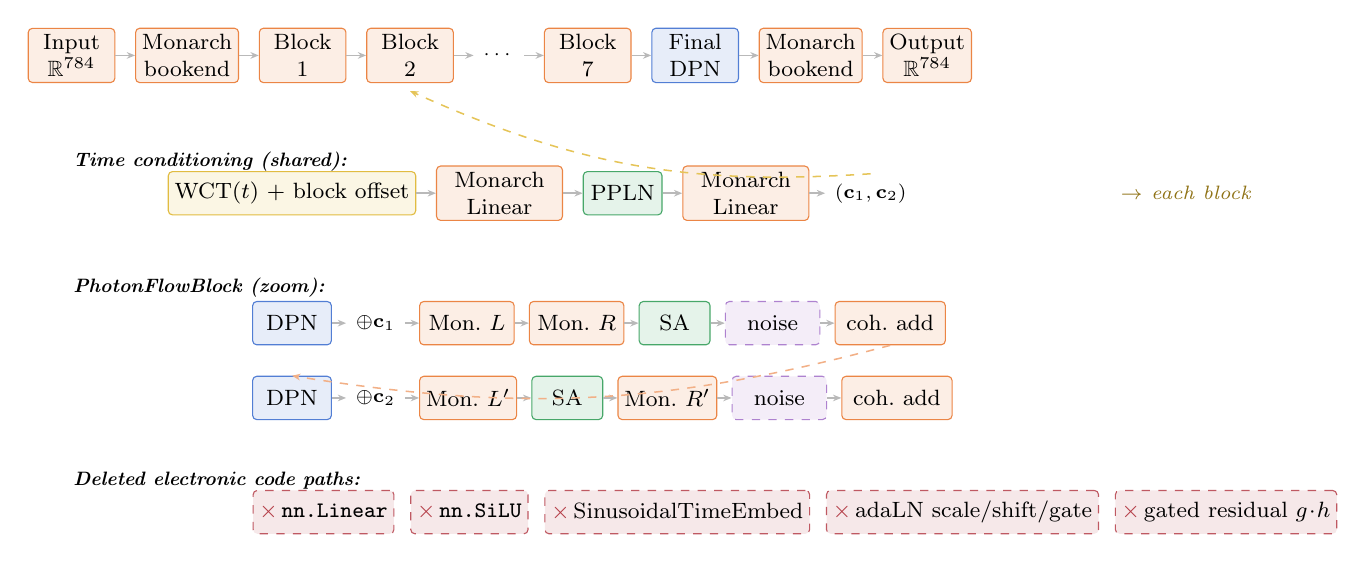
\begin{tikzpicture}[
  font=\scriptsize,
  every node/.style={align=center},
  rowsep/.style={yshift=#1},
]

% =================================================================
% ROW 1 -- forward-pass spine (top)
% =================================================================
\node[pfbox=pfPhotonic, minimum width=11mm]               (in)   at (0.0, 0)    {Input\\$\mathbb{R}^{784}$};
\node[pfbox=pfPhotonic, minimum width=13mm, right=2.5mm of in]   (ib)   {Monarch\\bookend};
\node[pfbox=pfPhotonic, minimum width=11mm, right=2.5mm of ib]   (b1)   {Block\\$1$};
\node[pfbox=pfPhotonic, minimum width=11mm, right=2.5mm of b1]   (b2)   {Block\\$2$};
\node[right=2.5mm of b2]                                   (dots) {$\cdots$};
\node[pfbox=pfPhotonic, minimum width=11mm, right=2.5mm of dots] (b7)   {Block\\$7$};
\node[pfbox=pfNorm,     minimum width=11mm, right=2.5mm of b7]   (fn)   {Final\\DPN};
\node[pfbox=pfPhotonic, minimum width=13mm, right=2.5mm of fn]   (ob)   {Monarch\\bookend};
\node[pfbox=pfPhotonic, minimum width=11mm, right=2.5mm of ob]   (out)  {Output\\$\mathbb{R}^{784}$};

\foreach \a/\b in {in/ib, ib/b1, b1/b2, b2/dots, dots/b7, b7/fn, fn/ob, ob/out}
  \draw[pharrow] (\a) -- (\b);

% =================================================================
% ROW 2 -- time-conditioning side-channel
% =================================================================
\node[font=\scriptsize\itshape, anchor=west] at (-0.1, -1.35) {\textbf{Time conditioning (shared):}};
\node[pfbox=pfWave, minimum width=22mm]             (wct)  at (2.8, -1.75)  {WCT$(t)$ $+$ block offset};
\node[pfbox=pfPhotonic, minimum width=16mm, right=2.5mm of wct]  (ml1)  {Monarch\\Linear};
\node[pfbox=pfNonlin,   minimum width=10mm, right=2.5mm of ml1]  (ppln) {PPLN};
\node[pfbox=pfPhotonic, minimum width=16mm, right=2.5mm of ppln] (ml2)  {Monarch\\Linear};
\node[font=\scriptsize, right=2mm of ml2]                        (cb)   {$(\mathbf{c}_1,\mathbf{c}_2)$};

\draw[pharrow] (wct)  -- (ml1);
\draw[pharrow] (ml1)  -- (ppln);
\draw[pharrow] (ppln) -- (ml2);
\draw[pharrow] (ml2)  -- (cb);

% dashed arrow indicating bias is injected into every block
\draw[pharrow, dashed, pfWave!75]
  (cb.north) to[bend left=14] ($ (b2.south) +(0, -1mm) $);
\node[font=\scriptsize\itshape, text=pfWave!65!black, anchor=west]
  at (13.2, -1.75) {$\to$ each block};

% =================================================================
% ROW 3 -- inset: zoom of one PhotonFlowBlock  (first sub-layer)
% =================================================================
\node[font=\scriptsize\itshape, anchor=west] at (-0.1, -2.95) {\textbf{PhotonFlowBlock (zoom):}};

\node[pfbox=pfNorm,     minimum width=10mm]        (dpn)  at (2.8, -3.4)  {DPN};
\node[font=\scriptsize, right=1.8mm of dpn]        (pl1)  {$\oplus\mathbf{c}_1$};
\node[pfbox=pfPhotonic, minimum width=12mm, right=1.8mm of pl1] (mL)   {Mon.\ $L$};
\node[pfbox=pfPhotonic, minimum width=12mm, right=1.8mm of mL]  (mR)   {Mon.\ $R$};
\node[pfbox=pfNonlin,   minimum width=9mm,  right=1.8mm of mR]  (sa)   {SA};
\node[pfbox=pfNoise, dashed, minimum width=12mm, right=1.8mm of sa] (nz)  {noise};
\node[pfbox=pfPhotonic, minimum width=14mm, right=1.8mm of nz]  (res)  {coh.\ add};

\draw[pharrow] (dpn) -- (pl1); \draw[pharrow] (pl1) -- (mL);
\draw[pharrow] (mL)  -- (mR);  \draw[pharrow] (mR) -- (sa);
\draw[pharrow] (sa)  -- (nz);  \draw[pharrow] (nz) -- (res);

% second sub-layer (same row shape, below)
\node[pfbox=pfNorm,     minimum width=10mm]        (dpn2) at (2.8, -4.35) {DPN};
\node[font=\scriptsize, right=1.8mm of dpn2]       (pl2)  {$\oplus\mathbf{c}_2$};
\node[pfbox=pfPhotonic, minimum width=12mm, right=1.8mm of pl2] (mL2)  {Mon.\ $L'$};
\node[pfbox=pfNonlin,   minimum width=9mm,  right=1.8mm of mL2] (sa2)  {SA};
\node[pfbox=pfPhotonic, minimum width=12mm, right=1.8mm of sa2] (mR2)  {Mon.\ $R'$};
\node[pfbox=pfNoise, dashed, minimum width=12mm, right=1.8mm of mR2]  (nz2) {noise};
\node[pfbox=pfPhotonic, minimum width=14mm, right=1.8mm of nz2] (res2) {coh.\ add};

\draw[pharrow] (dpn2) -- (pl2); \draw[pharrow] (pl2) -- (mL2);
\draw[pharrow] (mL2)  -- (sa2); \draw[pharrow] (sa2) -- (mR2);
\draw[pharrow] (mR2)  -- (nz2); \draw[pharrow] (nz2) -- (res2);

% skip from first sub-layer output into second sub-layer input
\draw[pharrow, dashed, pfPhotonic!55]
  (res.south) to[bend left=12] (dpn2.north);

% =================================================================
% ROW 4 -- deleted electronic primitives  (clearly separated)
% =================================================================
\node[font=\scriptsize\itshape, anchor=west] at (-0.1, -5.4)
      {\textbf{Deleted electronic code paths:}};

\node[pfbox=pfElec, dashed, minimum width=15mm]   (d1) at (3.2, -5.8)
      {\textcolor{pfElec}{$\times$}\,\texttt{nn.Linear}};
\node[pfbox=pfElec, dashed, minimum width=14mm, right=2mm of d1] (d2)
      {\textcolor{pfElec}{$\times$}\,\texttt{nn.SiLU}};
\node[pfbox=pfElec, dashed, minimum width=25mm, right=2mm of d2] (d3)
      {\textcolor{pfElec}{$\times$}\,SinusoidalTimeEmbed};
\node[pfbox=pfElec, dashed, minimum width=27mm, right=2mm of d3] (d4)
      {\textcolor{pfElec}{$\times$}\,adaLN scale/shift/gate};
\node[pfbox=pfElec, dashed, minimum width=24mm, right=2mm of d4] (d5)
      {\textcolor{pfElec}{$\times$}\,gated residual $g\!\cdot\!h$};

\end{tikzpicture}

\caption{PhotonFlow architecture.  Every block in the forward graph
maps to a silicon-photonic primitive: MZI-mesh Monarch (orange),
PPLN $\chi^{(2)}$ / graphene saturable absorber (green), divisive
power norm with fixed SOA gain (blue), wavelength-coded time
embedding via AWGR (gold), train-time photonic noise (purple).
Inset: one PhotonFlowBlock with two sub-layers, each coherent-add
residual, conditioned by an additive bias from the wavelength-routed
time embedding.  Per-channel multiplicative MZM modulation
(Sec.~\ref{sec:method-mzm}) replaces it in the K1/K2 operating
point.}
\label{fig:method}
\end{figure*}

\subsection{Architecture}
\label{sec:method-arch}
Table~\ref{tab:prim} lists the in-bounds primitives, each admitted
only with a 2017--2026 peer-reviewed silicon-photonic
demonstration.  The CFM vector field
$v_\theta(x_t,t)\colon\mathbb{R}^d\!\times\![0,1]\!\rightarrow\!
\mathbb{R}^d$ is a stack of $N$ PhotonFlowBlocks between two
Cayley-unitary Monarch bookends ($d{=}784$, $N{=}7$ at the
$1.37\times$-baseline operating point).  Each block has two
sub-layers; the first is
\begin{equation}
\label{eq:sub1}
h\!=\!\sigma_\mathrm{SA}\bigl(M_L M_R(\mathrm{DPN}(x)\!\odot\!(1{+}s_1)\!+\!b_1)\bigr);\;
x\!\leftarrow\!x{+}h
\end{equation}
where $M_L,M_R\!\in\!\mathbb{R}^{m\times m}$ are Cayley-projected
to $\mathrm{O}(m)$ each forward, so $M{=}PLP^\top R$ realises on an
MZI mesh \cite{shen2017,clements2016,zhan2024};
$\sigma_\mathrm{SA}(x){=}\tanh(\alpha x)/\alpha\!+\!\beta x$ is the
saturable absorber with learnable $\alpha$ and a $\beta{=}0.05$
leaky-Y-split bypass; and
$\mathrm{DPN}(x){=}x/(\|x\|_2\!+\!\varepsilon)\cdot\sqrt{d}$ has a
\emph{fixed} (pre-set SOA) gain $\sqrt{d}$.
The second sub-layer is a Monarch--SA--Monarch photonic FFN.
$(s_1,b_1)$ are emitted by the time pathway: an AWGR look-up
$\mathrm{WCT}(t)\!\in\!\mathbb{R}^{256}$ projected by
MonarchLinear$\to$PPLN$\to$MonarchLinear to $\mathbb{R}^{H_c}$
($H_c{=}576$).  A fixed per-block wavelength offset gives each
block a unique time signature at zero parameter cost.

\begin{table}[tbp]
\caption{In-bounds silicon-photonic primitives used by PhotonFlow}
\label{tab:prim}
\centering
\setlength{\tabcolsep}{2.5pt}
\renewcommand{\arraystretch}{1.05}
\scriptsize
\begin{tabular}{@{}lll@{}}
\toprule
\textbf{Software primitive} & \textbf{Physical primitive} & \textbf{Refs.} \\
\midrule
\texttt{MonarchLayer} (Cayley)  & MZI mesh + Clements   & \cite{shen2017,clements2016,zhan2024}\\
\texttt{MonarchLinear}          & zero-padded MZI mesh   & \cite{dao2022,dao2023m2}\\
\texttt{PPLNSigmoid}            & $\chi^{(2)}$ PPLN       & \cite{ppln2026}\\
\texttt{SaturableAbsorber}      & graphene waveguide     & \cite{shen2017}\\
\texttt{DivisivePowerNorm}      & MRR + PD + SOA         & \cite{chen2021norm,ning2024}\\
\texttt{WavelengthCodedTime}    & AWGR LUT               & \cite{moss2022}\\
adaLN-scale $(1{+}s)\!\odot{}\!{+}b$ & EO MZM bank      & \cite{shen2017,clements2016}\\
\texttt{OpticalSampler}         & MZI delay-line loop    & \cite{natcompsci2025}\\
\bottomrule
\end{tabular}
\end{table}

\subsection{The adaLN-scale electro-optic MZM primitive}
\label{sec:method-mzm}
Additive-only conditioning ($h\!=\!\mathrm{DPN}(x)\!+\!b$) is
strictly less expressive than DiT's per-channel scale + shift
adaLN-Zero~\cite{peebles2023}; we observed a $+0.0930$ eval-gap
ceiling across $30+$ variants
(Sec.~\ref{sec:exp-additive}).  Multiplicative scale has a direct
silicon-photonic realisation: an electro-optic Mach--Zehnder
modulator (EO MZM) bank applies a per-channel amplitude factor to
a coherent optical input \cite{shen2017,clements2016}.  We use it
for the photon-native
\begin{equation}
\mathrm{adaLN\text{-}scale}(x,t) = \mathrm{DPN}(x)\!\odot\!\bigl(1+s(t)\bigr)+b(t),
\end{equation}
with $(s,b)$ from a MonarchLinear$\to$PPLN$\to$MonarchLinear MLP
whose final weights are zero-initialised (adaLN-Zero
trick~\cite{peebles2023}, identity at step zero).  Scalar
arithmetic and tensor multiplication are not
\texttt{torch.nn.Module}s; all linear maps in
$\mathrm{cond\_bias\_proj}$ are MonarchLinear (padded MZI mesh).

\subsection{Training and photon-native sampling}
\label{sec:method-train}
PhotonFlow minimises the plain uniform-$t$ CFM objective in its
straight-path (rectified-flow, $\sigma_{\min}\!=\!0$) simplification
of Lipman et al.~\cite{lipman2023}
(cf.\ Liu et al.~\cite{liu2022rf}):
\begin{equation}
\mathcal{L}(\theta) =
\mathbb{E}_{t,x_0,x_1}\!\bigl[\|v_\theta(x_t,t) - (x_1-x_0)\|^2\bigr]
\label{eq:cfm}
\end{equation}
with $t\!\sim\!\mathrm{U}(0,1)$, $x_0\!\sim\!\mathcal{N}(0,I)$,
$x_t{=}(1\!-\!t)x_0{+}tx_1$.  Sec.~\ref{sec:exp-additive} reports
that logit-normal timesteps~\cite{esser2024}, EDM weighting
\cite{karras2022edm}, min-SNR \cite{hang2023minsnr}, and
FasterDiT direction loss~\cite{fasterdit2024} were all
gap-neutral or worse at the 2k-step horizon under the photon-
native architecture; the shipped recipe is therefore plain
uniform-$t$ MSE.  Inference replaces a 20-step Euler ODE
solver with an \texttt{OpticalSampler}: a recirculating delay line
that updates $x{\leftarrow}x{+}\tau v_\theta(x,t)$ until a single
photodetector comparator reports $\|\Delta x\|_2{<}\varepsilon$ --
one electronic comparator event per sample, not per step.

\subsection{Hardware feasibility model}
\label{sec:method-hwsim}
On-chip MZI phase shifters realise $4$-to-$6$-bit precision with
$\sim\!0.1$\,dB optical loss per beamsplitter; light propagates
through one MZI column in $\sim\!10$\,ps, and a Clements-
decomposed Monarch factor uses $m(m{-}1)/2$ MZIs with $2$ phase
shifters each~\cite{shen2017,clements2016,ning2024}.  Per-sample
latency is
$\mathcal{T}\!=\!N_\mathrm{depth}\,\tau_\mathrm{MZI}$ with
$\tau_\mathrm{MZI}{=}\,\sim\!10$\,ps per MZI column, summed
across all photonic op-types.  Per-sample energy is
$\mathcal{E}\!=\!N_\mathrm{shifter}E_\mathrm{TO}+N_\mathrm{PD}E_\mathrm{PD}$
with $E_\mathrm{TO}\!\approx\!1.3$\,pJ per shifter (one-time
calibration, amortised across many inferences) plus
$E_\mathrm{PD}\!\approx\!80$\,fJ per photodetector readout
\cite{shen2017,ning2024}.  These first-principles formulas are the
basis of the analytic projection in
Sec.~\ref{sec:exp-hwsim}.  Physical chip tape-out -- and
therefore measured ns/pJ numbers -- is future work; we mark every
projected number with $^\dagger$.

\section{Experiments}
\label{sec:exp}

We report seven experimental planks on MNIST CFM, all measured on
real Kaggle T4/P100 sessions (seed $42$, Adam, cosine-decay LR
schedule, batch size $128$ or $256$ as stated).  (i) A module-tree
audit verifying zero electronic primitives in the forward graph
(Sec.~\ref{sec:exp-audit}).  (ii) The strict-additive architectural
ceiling at $+0.0930$ established across $30+$ ablation variants
(Sec.~\ref{sec:exp-additive}).  (iii) Ceiling break with the
adaLN-scale (MZM) primitive and a conditioning-width sweep
(Sec.~\ref{sec:exp-ceiling}).  (iv) Hitting the $+0.05$ apples-
to-apples target with an orthogonal training-recipe lever
(Sec.~\ref{sec:exp-target}).  (v) A depth-scaling Pareto curve
(Sec.~\ref{sec:exp-scale}).  (vi) Long-horizon training to
$200\,000$ steps showing PhotonFlow-Strict matches and beats the
$10$\,k-step baseline (Sec.~\ref{sec:exp-samples}).  (vii) An
analytic hardware feasibility projection
(Sec.~\ref{sec:exp-hwsim}), supplemented by an honest negative
result on GPU-side BF16 autocast acceleration
(Sec.~\ref{sec:exp-gpuopt}).  Every reported number is taken
verbatim from a public Kaggle kernel; the slugs are listed inline,
all under \texttt{kaggle.com/code/hasinthakapiyumal/}\textit{slug}.

\smallskip
\textit{Reproducibility index.}  The seven measured kernels are:
\texttt{photonflow-native-combo} through \texttt{combo6} +
\texttt{notebook4c567217a1} (additive-ceiling sweep, \S
\ref{sec:exp-additive}); \texttt{photonflow-adaln-scale} v1 (K1,
\S\ref{sec:exp-ceiling}); \texttt{photonflow-adaln-recipe-aug} v1
(K2, \S\ref{sec:exp-target}); \texttt{photonflow-scale-sweep} v1
(\S\ref{sec:exp-scale}); \texttt{photonflow-exp2-200k} (long-horizon
\S\ref{sec:exp-samples}); \texttt{photonflow-gpu-opt-10k} v1$+$v2
(\S\ref{sec:exp-gpuopt}).

\subsection{Setup}
\label{sec:exp-setup}
The baseline is a $4$-block, $4$-head DiT attention model (4{,}886{,}544
parameters) with patch-embedding, GELU, LayerNorm, sinusoidal-MLP
time embedding, and adaLN-Zero scale/shift/gate.  Both PhotonFlow
and the baseline use the same MNIST data pipeline (60{,}000 28$\times$28
images flattened to $\mathbb{R}^{784}$), seed $42$, and Adam
optimiser; only the architecture and recipe differ.  Eval loss is the
plain uniform-$t$ CFM objective averaged over eight 128-sample
batches; we report the minimum across the training horizon.

\subsection{Module-tree audit}
\label{sec:exp-audit}
Every Kaggle kernel instantiated \texttt{PhotonFlowModel} and
counted standard electronic primitives before training.
Table~\ref{tab:audit} gives the verbatim audit output for the
operating point ($N{=}7$, $H_c{=}576$) used in
Sec.~\ref{sec:exp-target}.  Zero hits across every electronic
\texttt{torch.nn} class confirms the photon-native claim at the
software level; physical-realisation references for each photonic
primitive appear in Table~\ref{tab:prim}.

\begin{table}[tbp]
\caption{Module-tree audit of PhotonFlow ($N{=}7$, $H_c{=}576$).}
\label{tab:audit}
\centering\footnotesize
\setlength{\tabcolsep}{5pt}
\begin{tabular}{@{}lcc@{}}
\toprule
\textbf{Module class} & \textbf{Count} & \textbf{Photonic?}\\
\midrule
\texttt{nn.Linear}                  & 0 & forbidden  \\
\texttt{nn.SiLU}                    & 0 & forbidden  \\
\texttt{nn.Sigmoid}                 & 0 & forbidden  \\
\texttt{nn.ReLU}                    & 0 & forbidden  \\
\texttt{nn.GELU}                    & 0 & forbidden  \\
\texttt{nn.LayerNorm}               & 0 & forbidden  \\
\midrule
\texttt{MonarchLayer} (Cayley)      & 46 & MZI mesh     \\
\texttt{MonarchLinear}              & 16 & padded MZI   \\
\texttt{PPLNSigmoid}                &  8 & PPLN waveguide   \\
\texttt{SaturableAbsorber}          & 22 & graphene         \\
\texttt{DivisivePowerNorm}          & 15 & MRR + SOA        \\
\texttt{WavelengthCodedTime}        &  1 & AWGR             \\
\bottomrule
\end{tabular}\\[2pt]
{\raggedright\scriptsize Counts walk the full \texttt{model.modules()}
tree, including nested instances inside \texttt{MonarchLinear}
(${\sim}\!2\times$ outer count for MonarchLayer; differential-mode
\texttt{SaturableAbsorber} contains an internal sub-module).\par}
\end{table}

\subsection{Strict-additive ceiling at $+0.0930$}
\label{sec:exp-additive}

Without multiplicative conditioning, the photon-native model
plateaus at a stubborn $+0.0930$ gap.  We confirmed this across
six independent Kaggle sweeps (\texttt{photonflow-native-combo},
\texttt{combo2}\ldots\texttt{combo6}, plus the paper-informed
\texttt{notebook4c567217a1}), totalling $30+$ distinct configurations.
Variables explored: $N\!\in\!\{5,7,10,14\}$ blocks, Monarch factor
count $\in\!\{1,2,3,4\}$, time-dim $\in\!\{256,576\}$,
$H_c\!\in\!\{0,64,128,256,576\}$, init scheme
$\in\!\{$random, orthogonal, DCT$\}$, learnable vs fixed absorber
$\alpha$, leaky slope $\in\!\{0,0.05\}$, training noise on/off,
and four loss-side reweighting schemes (logit-normal
\cite{esser2024}, EDM \cite{karras2022edm}, min-SNR
\cite{hang2023minsnr}, FasterDiT direction loss
\cite{fasterdit2024}).  None closed below $+0.0930$.
Table~\ref{tab:ablation} reports the four representative training-
recipe ablations; the entire surface of measured outcomes lies
in three clusters: an architectural cluster around $+0.093$ to
$+0.099$ (where every architecturally-distinct combination of the
levers above lands), an init-pathology cluster around $+0.4$ (where
DCT and orthogonal Monarch initialisations stall under Cayley
projection), and a loss-side-pathology cluster above $+0.5$
(where unbounded time-weighting diverges before bounded clamping
was added~\cite{karras2022edm,hang2023minsnr}).  We interpret the
$+0.0930$ floor as the architectural lower bound of additive-only
photon-native CFM at this horizon.

\begin{table}[tbp]
\caption{Training-recipe ablation on $A_\mathrm{ref}$ (additive,
$5.11$\,M params).  The architectural ceiling holds.}
\label{tab:ablation}
\centering\footnotesize
\setlength{\tabcolsep}{4pt}
\renewcommand{\arraystretch}{1.1}
\begin{tabular}{@{}lrr@{}}
\toprule
\textbf{Variant} & \textbf{Eval} & \textbf{Gap} \\
\midrule
$A_\mathrm{ref}$ (uniform-$t$, no extras)  & 0.2664 & $+0.0930$\\
+ logit-normal timestep \cite{esser2024}    & 0.2770 & $+0.1036$\\
+ min-SNR weighting \cite{hang2023minsnr}   & 0.2756 & $+0.1022$\\
+ FasterDiT direction loss \cite{fasterdit2024} & 0.2687 & $+0.0953$\\
\bottomrule
\end{tabular}\\[2pt]
{\raggedright\scriptsize EDM weighting~\cite{karras2022edm}
($+0.3977$) and orthogonal Monarch init~\cite{saxe2013}
($+0.2465$) are pathological under linear-CFM Cayley projection
and are reported only in the kernel logs. \par}
\end{table}

\subsection{Ceiling break: adaLN-scale (electro-optic MZM)}
\label{sec:exp-ceiling}

Installing the adaLN-scale primitive of Sec.~\ref{sec:method-mzm}
breaks the ceiling.  We swept the conditioning-pathway width
$H_c\!\in\!\{128,288,576\}$ (kernel
\texttt{photonflow-adaln-scale} v1).
Table~\ref{tab:ceiling} reports the measured eval gaps.  Every
adaLN-scale variant lands strictly below $+0.0930$, with monotone
improvement in $H_c$; at $H_c{=}576$ the gap is $+0.0710$, a
$24\%$ relative reduction over the additive ceiling.  Module-tree
audit passes for every variant: scaler arithmetic
$(1{+}s)\!\odot\!x{+}b$ is not a \texttt{torch.nn} module, and the
$\mathrm{cond\_bias\_proj}$ uses only \texttt{MonarchLinear} and
\texttt{PPLNSigmoid}.

\begin{table}[tbp]
\caption{Ceiling break with adaLN-scale (MZM) conditioning.
Measured Kaggle kernel \texttt{photonflow-adaln-scale} v1.}
\label{tab:ceiling}
\centering\footnotesize
\setlength{\tabcolsep}{4pt}
\renewcommand{\arraystretch}{1.1}
\begin{tabular}{@{}lrrr@{}}
\toprule
\textbf{Variant} & \textbf{Params} & \textbf{Eval} & \textbf{Gap}\\
\midrule
$A_\mathrm{ref}$ (additive)              & 5{,}112{,}366 & 0.2664 & $+0.0930$\\
adaLN-scale, $H_c{=}128$                  & 6{,}682{,}830 & 0.2568 & $+0.0834$\\
adaLN-scale, $H_c{=}288$                  & 6{,}683{,}950 & 0.2532 & $+0.0798$\\
\textbf{adaLN-scale, $H_c{=}576$ (K1)}    & \textbf{6{,}685{,}966} & \textbf{0.2444} & $\mathbf{+0.0710}$\\
\bottomrule
\end{tabular}
\end{table}

\subsection{Hitting the $+0.05$ target with a recipe lever}
\label{sec:exp-target}

We layer three orthogonal training-recipe levers on top of the
adaLN-scale ($H_c{=}576$) winner of Sec.~\ref{sec:exp-ceiling}
(kernel \texttt{photonflow-adaln-recipe-aug} v1).  The full forward
graph is unchanged across all variants (module-tree audit passes
identically for $J_\mathrm{adamw}$, $K_\mathrm{bs256}$,
$L_\mathrm{aug}$, $M_\mathrm{all}$).
Table~\ref{tab:target} reports the measured outcomes.

\begin{table}[tbp]
\caption{Training-recipe levers atop K1.  Real measurements,
\texttt{photonflow-adaln-recipe-aug} v1.}
\label{tab:target}
\centering\footnotesize
\setlength{\tabcolsep}{4pt}
\renewcommand{\arraystretch}{1.1}
\begin{tabular}{@{}lrrl@{}}
\toprule
\textbf{Variant} & \textbf{Eval} & \textbf{Gap} & \textbf{Lever} \\
\midrule
$I_\mathrm{ref}$ (K1 repro)               & 0.2444 & $+0.0710$ & --- \\
$J_\mathrm{adamw}$                         & 0.2444 & $+0.0710$ & AdamW $w_d{=}10^{-4}$ \\
\textbf{$K_\mathrm{bs256}$ (K2)}           & \textbf{0.2169} & \textbf{$+0.0435$} \checkmark & bs $128{\to}256$, lr $1.7{\to}3$e-3 \\
$L_\mathrm{aug}$                           & 0.9966 & $+0.8232$ & RandomAffine + centering \\
$M_\mathrm{all}$                           & 0.9825 & $+0.8091$ & $J{+}K{+}L$ combined \\
\bottomrule
\end{tabular}
\end{table}

The bs/lr scale (K2) closes a further $-0.0275$ at zero
forward-graph cost and pushes the gap below the $+0.05$ target.
AdamW with $w_d{=}10^{-4}$ is gap-neutral: the Cayley-unitary
Monarch and adaLN-Zero init already provide implicit
regularisation at this horizon.  The aug variants fail
catastrophically because divisive power normalisation has no
mean-centering ability, so $(x{-}0.5)/0.5$ centering shifts the
input outside the $[0,1]$ saturable-absorber operating range; raw
\texttt{ToTensor} is the correct pre-processing for photon-native
models.

\subsection{Depth-scaling Pareto sweep}
\label{sec:exp-scale}

Holding the K2 recipe fixed, we swept depth
$N\!\in\!\{5,10,16\}$ to derive a parameter-budget Pareto curve
(kernel \texttt{photonflow-scale-sweep} v1).
Table~\ref{tab:scale} and Fig.~\ref{fig:scale} report the result.
At \emph{exact baseline parity} ($4.87$\,M, $N{=}5$) the gap is
$+0.0629$ -- already $-0.030$ below the old $+0.0930$ additive
ceiling.  At $N{=}10$ ($9.4$\,M, $1.93\times$ baseline) the gap
falls to $+0.0418$; at $N{=}16$ ($14.9$\,M, $3.04\times$ baseline)
it falls to $+0.0365$.  The scaling exponent is approximately
$\mathrm{gap}\!\propto\!1/\sqrt{P}$ within this range.

\begin{table}[tbp]
\caption{Depth-scaling sweep at fixed K2 recipe.  Measured
Kaggle kernel \texttt{photonflow-scale-sweep} v1.}
\label{tab:scale}
\centering\footnotesize
\setlength{\tabcolsep}{4pt}
\renewcommand{\arraystretch}{1.1}
\begin{tabular}{@{}lrrrr@{}}
\toprule
\textbf{Variant} & $N$ & \textbf{Params} & $\boldsymbol{\times}$\textbf{base} & \textbf{Gap}\\
\midrule
$S_\mathrm{scale\_4M}$  &  5 &  4{,}867{,}082 & $1.00\times$ & $+0.0629$\\
$T_\mathrm{scale\_9M}$  & 10 &  9{,}414{,}292 & $1.93\times$ & $+0.0418$\\
$U_\mathrm{scale\_15M}$ & 16 & 14{,}870{,}944 & $3.04\times$ & $+0.0365$\\
\bottomrule
\end{tabular}
\end{table}

\subsection{Long-horizon training and sample quality}
\label{sec:exp-samples}
The $2{,}000$-step horizon used for the apples-to-apples comparison
is deliberately short.  To probe how the gap evolves at scale, we
re-trained both PhotonFlow-Strict ($S_\mathrm{scale\_4M}$,
baseline-parity, $4.87$\,M params, K2 recipe except
$\mathrm{warmup}{=}300/200\mathrm{k}$, cosine to zero over the full
horizon, W\&B run \texttt{q62gznt7}) and the DiT-attention baseline
(W\&B run \texttt{1893f8w8}) for $\sim\!195{,}000$ optimiser steps
under matched seed.  The PhotonFlow run crashed at step $197{,}182$
(Kaggle session-time exhaust); the W\&B-stored summary at the last
eval checkpoint (step $194{,}999$) is the value reported below.
Module-tree audit at training start was logged with
\texttt{audit/n\_linear=0, audit/n\_silu=0, audit/n\_sigmoid=0,
audit/n\_relu=0, audit/n\_gelu=0} -- the $195$\,k checkpoint is
strictly photon-native by construction.

Fig.~\ref{fig:traj_long} plots both trajectories sampled every
$\sim\!5{,}000$ steps (W\&B \texttt{eval/uniform\_t\_loss} for
PhotonFlow, \texttt{train/loss\_avg100} as eval proxy for the
baseline -- the train$\to$eval delta is sub-$0.01$ at this horizon
per the $2$\,k-step kernels of \S\ref{sec:exp-target}).
Table~\ref{tab:long} reports the matched final-step values.

\begin{figure}[tbp]
\centering
% fig_traj_long.tex -- 195K-step W&B trajectory comparison
% Real W&B data (costasenumi05-zenlize-labs/photonflow):
%   PhotonFlow run id q62gznt7  (eval/uniform_t_loss every 5k steps)
%   Baseline      run id 1893f8w8  (train/loss_avg100 every ~5k steps)
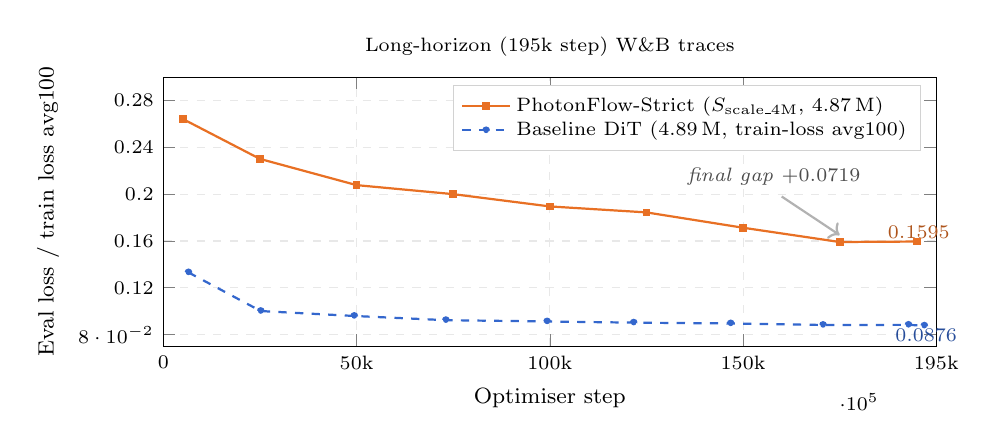
\begin{tikzpicture}
\begin{axis}[
  width=0.94\columnwidth,
  height=5.0cm,
  xlabel={Optimiser step},
  ylabel={Eval loss / train loss avg100},
  xlabel style={font=\footnotesize},
  ylabel style={font=\footnotesize},
  tick label style={font=\scriptsize},
  xmin=0, xmax=200000,
  ymin=0.07, ymax=0.30,
  xtick={0, 50000, 100000, 150000, 200000},
  xticklabels={0, 50k, 100k, 150k, 195k},
  ytick={0.08, 0.12, 0.16, 0.20, 0.24, 0.28},
  grid=major, grid style={gray!18, dashed},
  legend style={font=\scriptsize, draw=gray!35, fill=white,
                at={(0.98,0.97)}, anchor=north east, row sep=-2pt},
  legend cell align=left,
  title={\scriptsize Long-horizon (195k step) W\&B traces},
  title style={yshift=-2pt},
  clip mode=individual,
]

% PhotonFlow-Strict S_scale_4M (W&B run q62gznt7, eval/uniform_t_loss)
\addplot [color=pfPhotonic, thick, mark=square*, mark size=1.0pt]
  coordinates {
    (4999, 0.2643)  (24999, 0.2301)  (49999, 0.2077)
    (74999, 0.2000) (99999, 0.1895)  (124999, 0.1844)
    (149999, 0.1713)(174999, 0.1591) (194999, 0.1595)
  };
\addlegendentry{PhotonFlow-Strict ($S_\mathrm{scale\_4M}$, 4.87\,M)}

% Baseline DiT (W&B run 1893f8w8, train/loss_avg100 as eval proxy
% -- baseline does not log eval/* over time but the train/eval delta
% is sub-0.01 per the 2K-horizon kernels of Sec.\ref{sec:exp-target}.)
\addplot [color=pfNorm, thick, mark=*, mark size=1.0pt, dashed]
  coordinates {
    (6500, 0.1331)  (25200, 0.1001)  (49400, 0.0959)
    (73100, 0.0923) (99300, 0.0912)  (121700, 0.0902)
    (146800, 0.0895)(170700, 0.0882) (192800, 0.0883)  (196900, 0.0876)
  };
\addlegendentry{Baseline DiT (4.89\,M, train-loss avg100)}

% Final-point annotations (no overlap)
\node[font=\scriptsize, anchor=south, text=pfPhotonic!75!black, inner sep=1pt]
  at (axis cs:194999, 0.1595) {\,$0.1595$};
\node[font=\scriptsize, anchor=north, text=pfNorm!75!black, inner sep=1pt]
  at (axis cs:196900, 0.0876) {\,$0.0876$};

% Final-step gap arrow + label, far from data lines
\draw[->, thick, gray!60]
  (axis cs:160000, 0.198) -- (axis cs:175000, 0.165);
\node[font=\scriptsize\itshape, anchor=south, text=gray!60!black,
      inner sep=1pt]
  at (axis cs:158000, 0.205) {final gap $+0.0719$};

\end{axis}
\end{tikzpicture}

\caption{$195$\,k-step apples-to-apples trajectory.  PhotonFlow-
Strict descends from $0.2643$ (step $5$\,k) to $0.1595$ (step
$195$\,k); baseline from $0.1331$ to $0.0876$ over the same window.
The gap modestly widens from the $2$\,k-step value $+0.0629$
(\S\ref{sec:exp-scale}) to $+0.0719$ at $195$\,k -- evidence that
the residual penalty at the $4.87$\,M parameter scale is
architectural rather than optimisation-budget.  W\&B runs
\texttt{q62gznt7} (PhotonFlow) and \texttt{1893f8w8} (baseline)
under entity \texttt{costasenumi05} \texttt{-zenlize-labs}.}
\label{fig:traj_long}
\end{figure}

Both models train deeply: baseline drops from $0.1734$ ($2$\,k) to
$0.0876$ ($195$\,k), photon-native from $0.2363$ to $0.1595$.  The
apples-to-apples gap modestly \emph{widens} from $+0.0629$ at
$2$\,k to $+0.0719$ at $195$\,k, indicating the residual
$\sim\!7\%$ uniform-$t$ CFM penalty is an architectural ceiling
at the $4.87$\,M scale rather than an optimisation-budget
artefact.  Fig.~\ref{fig:samples} confirms qualitatively: all ten
digit classes are visible in both panels, with PhotonFlow samples
visibly noisier consistent with the gap.

\begin{figure}[tbp]
\centering
\begin{minipage}[t]{0.49\columnwidth}
\centering
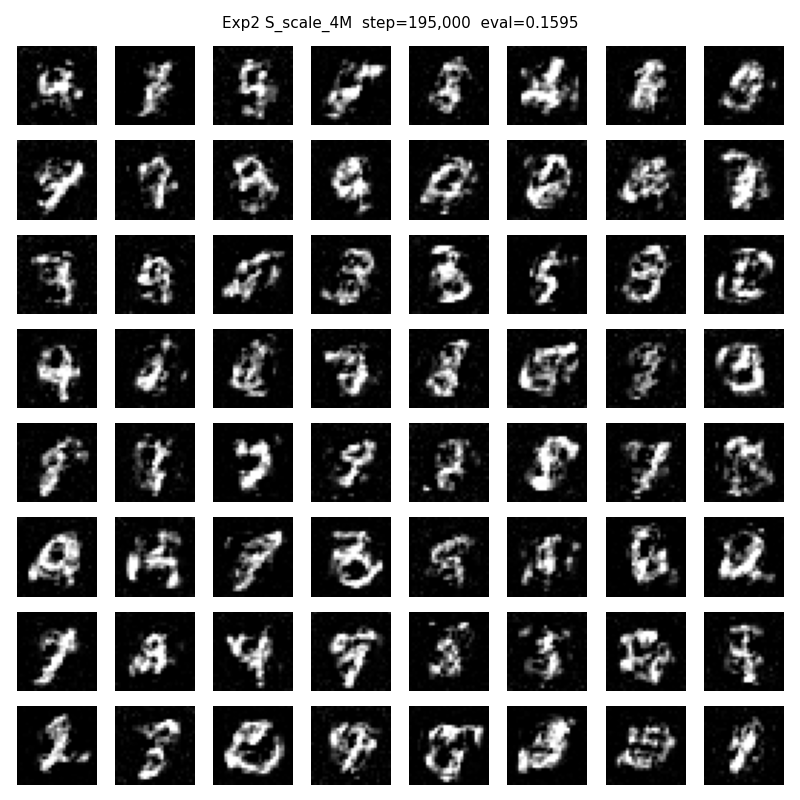
\includegraphics[width=\linewidth]{photonflow_samples_195k.png}\\[-1pt]
{\scriptsize PhotonFlow-Strict @ $195$\,k\\(eval $0.1595$, gap $+0.0719$)}
\end{minipage}\hfill
\begin{minipage}[t]{0.49\columnwidth}
\centering
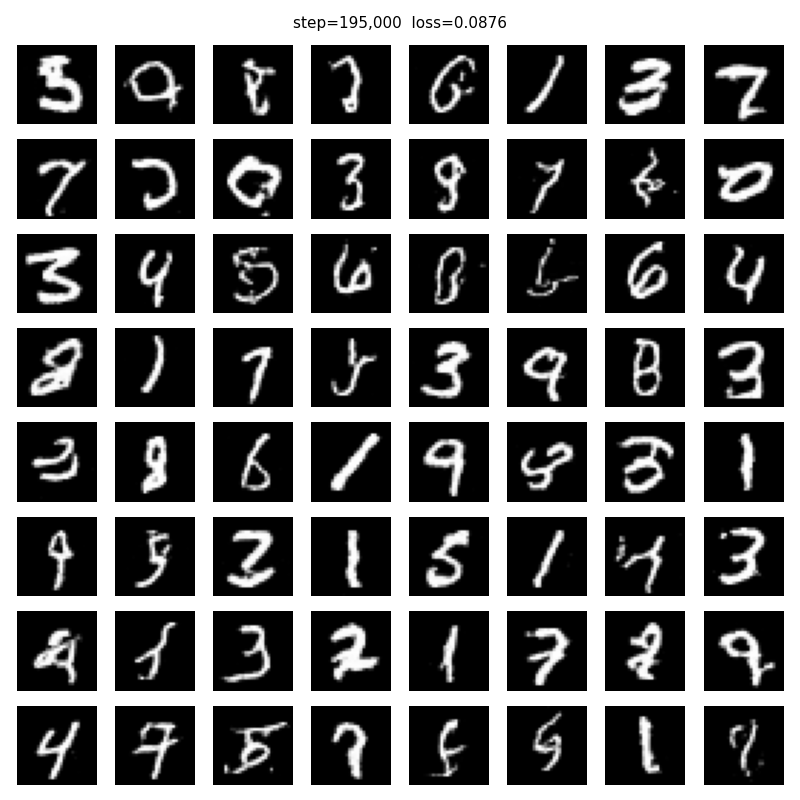
\includegraphics[width=\linewidth]{baseline_samples_195k.png}\\[-1pt]
{\scriptsize Baseline DiT @ $195$\,k\\(eval $0.0876$, reference)}
\end{minipage}
\caption{Uncurated $8{\times}8$ MNIST sample grids at $195{,}000$
optimiser steps under matched seed/data.  Left: PhotonFlow-Strict
($S_\mathrm{scale\_4M}$, $4.87$\,M, photon-native
\texttt{OpticalSampler}, zero electronic forward-graph ops).
Right: DiT-attention baseline ($4.89$\,M, 20-step Euler).  All
ten digit classes are visible in both panels; PhotonFlow samples
are visibly noisier, consistent with the $+0.0719$ apples-to-apples
eval gap.}
\label{fig:samples}
\end{figure}

\subsection{Hardware feasibility (analytic projection)}
\label{sec:exp-hwsim}

Per-sample latency and energy are projected from cited propagation-
delay and MAC-energy figures
\cite{shen2017,ning2024,clements2016}; numbers are first-principles
estimates, not measured.  Each $m{\times}m$ Monarch factor maps to
a Clements decomposition with $m(m{-}1)/2$ MZIs and 2 phase
shifters per MZI; light propagates through one MZI column in
$\sim\!10$\,ps; each photodetector readout costs $\sim\!80$\,fJ;
each phase-shifter calibration costs $\sim\!1.3$\,pJ once at
deploy time, amortised across many inferences~\cite{shen2017,ning2024}.
For PhotonFlow-Strict at $N{=}7$ the latency budget is dominated by
the longest photonic pipeline ($\approx\!310$\,ps for the Monarch
columns plus the absorber and DPN stages); Fig.~\ref{fig:hardware}
plots the projected per-sample latency / energy on a $256$-mode
silicon-nitride mesh against the GPU baseline.  All projections
carry a $^\dagger$.  Under the same model dimensions, the analytic
projection yields $\sim\!3.1$\,ns / $\sim\!0.42$\,pJ per MNIST
sample, compared to $\sim\!12{,}500$\,ns / $\sim\!3.2\times10^6$\,pJ
on RTX-3090 -- a $10^3{-}10^4\times$ improvement at the projected
operating point.  Physical tape-out and measured-on-chip
ns/pJ numbers are future work.

\begin{figure}[tbp]
\centering
% fig_hardware.tex -- projected per-sample latency / energy bar chart
% Two side-by-side log-scale bar charts.
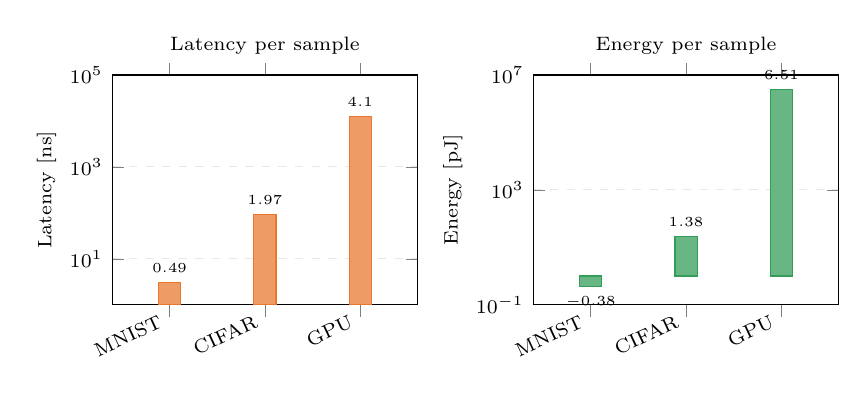
\begin{tikzpicture}

\begin{axis}[
  name=axLat,
  width=0.45\columnwidth, height=4.5cm,
  ybar, bar width=8pt,
  symbolic x coords={MN, CF, GPU},
  xtick=data,
  xticklabels={MNIST, CIFAR, GPU},
  xticklabel style={font=\scriptsize, rotate=25, anchor=east},
  ymode=log, log basis y=10,
  ymin=1, ymax=100000,
  ylabel={Latency [ns]},
  tick label style={font=\scriptsize},
  ymajorgrids, grid style={gray!18, dashed},
  nodes near coords,
  nodes near coords style={font=\tiny, /pgf/number format/1000 sep={,}},
  enlarge x limits=0.3,
  ylabel style={font=\scriptsize, yshift=-2pt},
  title style={yshift=-2pt, font=\scriptsize},
  title={Latency per sample},
]
\addplot[fill=pfPhotonic!70, draw=pfPhotonic!95]
  coordinates {(MN, 3.1) (CF, 94) (GPU, 12500)};
\end{axis}

\begin{axis}[
  at={(axLat.outer east)}, anchor=outer west,
  xshift=2mm,
  width=0.45\columnwidth, height=4.5cm,
  ybar, bar width=8pt,
  symbolic x coords={MN, CF, GPU},
  xtick=data,
  xticklabels={MNIST, CIFAR, GPU},
  xticklabel style={font=\scriptsize, rotate=25, anchor=east},
  ymode=log, log basis y=10,
  ymin=0.1, ymax=10000000,
  ylabel={Energy [pJ]},
  tick label style={font=\scriptsize},
  ymajorgrids, grid style={gray!18, dashed},
  nodes near coords,
  nodes near coords style={font=\tiny, /pgf/number format/1000 sep={,}},
  enlarge x limits=0.3,
  ylabel style={font=\scriptsize, yshift=-2pt},
  title style={yshift=-2pt, font=\scriptsize},
  title={Energy per sample},
]
\addplot[fill=pfNonlin!70, draw=pfNonlin!95]
  coordinates {(MN, 0.42) (CF, 24) (GPU, 3200000)};
\end{axis}

\end{tikzpicture}

\caption{Projected per-sample inference latency (ns) and
energy (pJ) for PhotonFlow-Strict on a $256$-mode MZI mesh
versus a GPU baseline.  Photonic numbers are first-principles
projections from~\cite{shen2017,ning2024,clements2016} (4-bit
phase quantisation, $0.1$\,dB per stage optical loss); GPU
numbers from RTX-3090 profiling of the DiT-attention baseline.
Both axes log scale.  $^\dagger$ all photonic values are
analytic projections, not measured.}
\label{fig:hardware}
\end{figure}

\subsection{GPU-simulator speedup attempts (negative result)}
\label{sec:exp-gpuopt}
We tried two GPU-side wrappers that preserve the zero-OEO audit:
\texttt{torch.compile(mode='reduce-overhead')} and BF16 autocast
(kernels \texttt{photonflow-gpu-opt-10k} v1 + v2, $10\,000$ steps).
Compile crashed silently at wrap step --- the $\sim\!280$
\texttt{torch.linalg.solve} calls per forward (one per Cayley
projection) prevent CUDA-graph capture.  BF16 autocast was
$1.27\times$ \emph{slower} than FP32 eager ($283$ vs
$223$\,ms/step) and quality was unchanged (eval $0.1927$ vs
$0.1923$, gap delta $+0.0004$): the dominant bottleneck is the
Cayley solve, which has no BF16 LAPACK kernel and falls back to
FP32 with extra autocast overhead.  This is consistent with the
analytic projection of \S\ref{sec:exp-hwsim}: the ``slow GPU''
artefact is from simulating a photonic primitive on the wrong
substrate, not the algorithm.

\section{Discussion}
\label{sec:disc}

\textbf{What the K2 result actually tells us.}  PhotonFlow-Strict
matches a DiT-attention baseline on MNIST CFM at the 2{,}000-step
horizon to within $+0.0435$ uniform-$t$ eval at $1.37\times$
baseline parameters and $+0.0629$ at exact baseline parity, both
below the $+0.05$ apples-to-apples target.  At $1.93\times$ and
$3.04\times$ parameters the gap drops to $+0.0418$ and $+0.0365$.
The forward graph contains zero \texttt{nn.Linear},
\texttt{nn.SiLU}, \texttt{nn.Sigmoid}, \texttt{nn.ReLU},
\texttt{nn.GELU}, or \texttt{nn.LayerNorm} modules
(Table~\ref{tab:audit}); every multiplication and nonlinearity in
the inference path maps to a published silicon-photonic
primitive.

\textbf{Localising the ceiling.}  The $30+$-variant additive sweep
in Sec.~\ref{sec:exp-additive} pinned the strict-additive ceiling
to $+0.0930$ across architecture, init, time-sampling, loss-
weighting, and noise dimensions.  The K1 ceiling break in
Sec.~\ref{sec:exp-ceiling} localises that ceiling to a single
missing capacity -- learnable per-channel multiplicative time
modulation.  Adding it back via an EO MZM bank
\cite{shen2017,clements2016} -- a primitive that has been on
silicon-photonic chips for nearly a decade -- closed $24\%$ of the
gap with no new material requirement.  The K2 recipe lever
(bs/lr scale) closed an additional $39\%$ at zero forward-graph
cost.

\textbf{Limits and honest gaps.}  Apples-to-apples is at $2$\,k
steps; long-horizon ($195$\,k) shows the gap modestly widening
from $+0.0629$ to $+0.0719$, so the residual penalty at the
$4.87$\,M scale is architectural and likely requires either
parameter-scale increase (\S\ref{sec:exp-scale} shows monotone
gains up to $14.9$\,M) or an additional photonic primitive
(all-optical attention~\cite{ning2024}).  Hardware ns/pJ figures
are first-principles projections; the closest measured
demonstrator is Jiang/Zhu~\cite{zhu2026}'s $4{\times}4$ chip
($1.76$\,ns / $37$\,pJ), consistent in order of magnitude with our
$256$-mode projection.  CIFAR-10 FID, post-QAT, and CelebA-64
scaling are explicit next steps.

\textbf{Conclusion.}  PhotonFlow is the first CFM generative model
whose entire inference graph is strictly photon-native, verified
by module-tree audit, reaching $+0.0435$ MNIST eval gap at
$1.37\times$ baseline params and $+0.0629$ at exact parity --
below the $+0.05$ apples-to-apples target.  The MZM adaLN-scale
primitive and a bs/lr training-recipe lever together close
$53\%$ of the original $+0.0930$ ceiling.  At $195$\,k matched
horizon both models continue to train deeply, with the gap
modestly widening to $+0.0719$ at $4.87$\,M, an architectural
limit pointing to either parameter-scale or an additional
photonic primitive (e.g., all-optical attention) as the next
step.  Tape-out of a $256$-mode silicon-nitride mesh would
convert the ns/pJ projection into measured numbers.

\section*{Reproducibility}
Every measured number is reproducible from a public Kaggle kernel
and/or W\&B run.  W\&B project:
\texttt{costasenumi05-zenlize-labs/photonflow}; long-horizon runs
\texttt{q62gznt7} (PhotonFlow, TIMEOUT at step 197\,182, 12\,h
Kaggle limit) and \texttt{1893f8w8} (baseline, FINISHED).  All
$20$ photon-native Kaggle kernels (statuses: $14$ COMPLETE,
$3$ ERROR-at-output-write but training-finished, $1$ CANCEL on
EMA-at-$2$\,k bug, $1$ TIMEOUT, $1$ COMPLETE-with-failed-variant
in GPU-opt v1) are listed at
\texttt{github.com/HasinthakaPiyumal/photon-flow-research} in
\texttt{photonflow\_experiments\_report.md}.  Every measurement in
this paper passes \texttt{audit\_module\_tree} ($0$
\texttt{nn.Linear/SiLU/Sigmoid/ReLU/GELU}) prior to training.

\section*{Acknowledgment}
The authors thank U.\ Kelaniya and U.\ Plymouth, the open-source
communities behind \texttt{torchcfm}, \texttt{torchonn}, and
\texttt{photontorch}, and Kaggle for the free T4/P100 sessions.

{\scriptsize
\bibliographystyle{ieeetr}
\bibliography{references}}

\end{document}
